\documentclass[UserManual.tex]{subfiles}
\begin{document}
\setcounter{section}{7}
\section{Tutorial}\label{sec:tutorial}

\subsection{Overview}
Template project directories and files are provided with the intention that the User will copy them to their own space, then use this as a foundation from which to embark on their own analysis. This directory includes information files, describing the parameter priors and the observables, that correspond to an artificial model that is also provided as a template. Working through the steps in this section constitutes a tutorial, both for running {\it Simplex Sampler} and for running {\it Smooth Emulator}.

This section describes the steps of how the User would
\begin{enumerate}\itemsep=0pt
\item Copy the required files from the template directory to the User's space, and compile the main programs.
\item Set up the information files describing the priors and observable names.
\item Run {\it Simplex Sampler} to generate the model-parameter values at which the full model will be trained.
\item Run a full model to generate the observables for each of the full-model runs.
\item Tune {\it Smooth Emulator} and write the coefficients to file.
\item Run a program that prompts the User for the coordinates of a point in parameter space, then returns the emulator prediction with its uncertainty.
\end{enumerate}

\subsection{Installation and Compilation}
Installation and compilation is described in Sec. \ref{sec:installation}. As was defined in that section, the tutorial will refer to three locations with the short hand:

\vspace*{0.2in}

\begin{tabular}{rl}\hline
{\tt \$\{GITHOME\_BAND\_SMOOTH\}} & \parbox{5in}{~\\Location of Git Repository, e.g.\\{\tt /Users/CarlosSmith/bandframework/software/SmoothEmulator}\\}\\
{\tt \$\{MY\_LOCAL\}} & \parbox{5in}{Can be placed anywhere. Executables are store in\\ {\tt \$\{MY\_LOCAL\}/bin} and main programs, and source codes for main\\ programs are found within {\tt \$\{MY\_LOCAL\}/software/main\_programs}\\}\\
{\tt \$\{MY\_PROJECT\}} & \parbox{5in}{Can be placed anywhere. Work spaces where parameter files, data, results and figures are created and stored. User may have several different such directories\\}\\
 \hline
\end{tabular}

At this point, the user should have established a personalized project directory by copying the {\tt \$\{GITHOME\_BAND\_SMOOTH\}/templates/} directory to a convenient location. For example,
{\tt
\begin{verbatim}
	% cp -r ${GITHOME_BAND_SMOTH}/templates /Users/CarlosSmith/mysmoothy
\end{verbatim}}
In this case {\tt \$\{MY\_LOCAL\}} will now refer to {\tt Users/CarlosSmith/mysmoothy/mylocal} and {\tt \$\{MY\_PROJECT\}} will now refer to a specific project at {\tt Users/CarlosSmith/mysmoothy/myproject}.

The User should have also compiled the main libraries
{\tt
\begin{verbatim}
   ${GITHOME_BAND_SMOOTH}/software% cmake .
   ${GITHOME_BAND_SMOOTH}/software% make
\end{verbatim}
}
and the main programs,
{\tt
\begin{verbatim}
   ${MY_LOCAL}/software% cmake .
   ${MY_LOCAL}/software% make
\end{verbatim}
}
This will compile all the main source programs in {\tt \$\{MY\_LOCAL\}/software/main\_programs/*.cc} and a ``fake'' full model to be used in the tutorial {\tt \$\{MY\_LOCAL\}/software/fakefulmodels/fakerhic.cc}. The repository was organized to encourage Users to edit any files in {\tt \$\{MY\_LOCAL\}/}. If the User wishes to restore any original files, a copy can be found at {\tt \$\{GITHOME\_BAND\_SMOOTH\}/templates/mylocal}.

Several executables should now appear in {\tt \$\{MY\_LOCAL\}/bin/}: {\tt simplex, smoothy\_tune, mcmc, smoothy\_testattrainingpts, smoothy\_testvsfullmodel, smoothy\_testvsfullmodelalt} and {\tt fakerhic}. The User might find it convenient to add {\tt \$\{MY\_LOCAL\}/bin} to their path. The reason these are compiled in the User's space, separate from the main libraries, is that the User may well wish to create their own main programs, and this arrangement allows the User to compile their own versions, while leaving the original programs from the templates directory and the lower-level source code unchanged. 

\subsection{Creating Necessary Info Files}
The User will run the software from the {\tt \$\{MY\_PROJECT\}/} directory. Before a User can run {\it Simplex Sampler} they must create information files that describe the model-parameter priors and list the observable names. Both files are need to be in the {\tt \$\{MY\_PROJECT\}} directory. The first file is {\tt smooth\_data/Info/modelpar\_info.txt}, which describes the model parameters and their priors. For the purposes of this tutorial, a file already exists,
{\tt
\begin{verbatim}
   compressibility         uniform  150   300
   etaovers                uniform  0.05  0.32
   initial_flow            uniform  0.3   1.2
   initial_screening       uniform  0.0   1.0
   quenching_length        uniform  0.5   2.0
   initial_epsilon         uniform  15.0  30.0
\end{verbatim}
}
Thus, the model has six parameters. The second entry in each line is either {\tt uniform} or {\tt gaussian}. If the entry is {\tt uniform}, the last two numbers represent the range of the uniform prior, $x_{\rm min}$ and $x_{\rm max}$. If the second entry is {\tt gaussian} the third entry represents the center of the Gaussian distribution and the fourth represents the width. For a full model, the User would replace this model with one appropriate for their own model.

The second file is {\tt smooth\_data/Info/observable\_info.txt}. This describes output values from the model. In the template, the provided file is
{\tt
\begin{verbatim}
   meanpt_pion    100      
   meanpt_kaon    200      
   meanpt_proton  300      
   Rinv           1.0      
   v2             0.2     
   RAA            0.5
\end{verbatim}
}
The first entry in each line simply provides the names of the observable which will be processed in the Bayesian analysis.  The second entry is used by {\tt Smooth Emulator} during tuning, but only if a Monte Carlo method is used, and then is only used to seed the Monte Carlo search. If the analytical method is used for tuning (which is recommended) this parameter is irrelevant (but still shoud be listed).

\subsection{Running {\it Simplex Sampler}}

Both {\it Simplex Sampler} and {\it Smooth Emulator} have options. These are provided in parameter files. For this tutorial, the provided parameter file is {\tt smooth\_data/smooth\_parameters/simplex\_parameters.txt}. The provided file is
{\tt
\begin{verbatim}
   #LogFileName    simplexlog.txt # comment out to direct output to screen
   Simplex_TrainType       2              # Must be 1 or 2             
   Simplex_ModelRunDirName modelruns      # Directory with training pt. info
\end{verbatim}
}
Because the first line is commented, the output of {\it Simplex Sampler} will be to the screen. Otherwise it would go to the specified file. By setting {\tt Simplex\_TrainType=1}, the sampler will choose $n+1$ training points, where $n=6$ is the number of model parameters. Each point corresponds to the vertices of an $n+1$ dimensional simplex.  Finally, the parameter {\tt Simplex\_ModelRunDirName} is set to ``{\tt modelruns}''. This informs {\tt Simplex Sampler} to write the coordinates of each training point and the corresponding observables in the directory {\tt smooth\_data/modelruns/}. Here, {\tt Simplex\_TrainType=2}, which adds points half-way between each pair of simplex points. These additonal points are then moved outward and the original simplex points are brought inward. This method has precisely the number of training points as the number of coefficients necessary for a quadratic fit. 

Now the user can run {\tt Simplex Sampler}, which must be run from the project directory. The only output is the number of training points.
 {\tt
\begin{verbatim}
   ${MY_PROJECT}/rhic% ${MY_LOCAL}/bin/simplex
   NTrainingPts=28
\end{verbatim}
}
If one had set {\tt Simplex\_TrainType}=1, only seven training points would have been created. The programs writes information about the training points in the {\tt smooth\_data/modelruns/} directory. Changing into that directory, there should now be 28 sub-directories, corresponding to the 28 training points: {\tt modelruns/run0}, {\tt modelruns/run1}, {\tt modelruns/run2}, {\tt modelruns/}$\cdots$. Each directory has one text file describing the training points. For example, the {\tt modelruns/run0/mod\_parameters.txt} file might be 
{\tt
\begin{verbatim}
   compressibility 190.282
   etaovers 0.14892
   initial_flow 0.664958
   initial_screening 0.426807
   quenching_length 1.16036
   initial_epsilon 21.7424
\end{verbatim}
}
This describes the six model parameters, which will serve as the input for the first full model run.  The next step will be to run the full model for the parameters in each directory. Thus for {\tt Simplex\_Traintype=1}, one would need 7 full-model runs, and for {\tt Simplex\_Traintype=2}, one would need to do 28 full-model runs. The corresponding observables will be written in the files {\tt smooth\_data/modelruns/runI/obs.txt}

\subsection{Running the Fake Full Model}
Once the training points have been generated, the user will run a full model based on the given structure, tailored to address their specific problem. For the tutorial, a fake full model is provided. It reads the model-parameter values in each {\tt smooth\_data/modelruns/runI/mod\_parameters.txt} file and writes the corresponding observables in {\tt smooth\_data/modelruns/runI/obs.txt}. The output should be as follows:
{\tt
\begin{verbatim}
   ${MY_PROJECT}/rhic% ${MY_LOCAL}/bin/fakerhic
   NTraining Pts=28
   NPars=6
\end{verbatim}
}
The output simply verifies the number of model parameters and the number of training points created by simplex.

Inspecting the {\tt smooth\_data/modelruns/run0/obs.txt} file,
{\tt
\begin{verbatim}
   meanpt_pion   418.821195  1.000000
   meanpt_kaon   715.592889  2.000000
   meanpt_proton 1079.482871 3.000000
   Rinv          5.004248    0.010000
   v2            0.178353    0.002000
   RAA           0.553416    0.005000
\end{verbatim}
}
The second entry of each line is the value of the specified observable for that specific training point. The last entry is the random uncertainty associated with the full model. This is only relevant if the model has random fluctuations, meaning the re-running the model at the same point might result in different output. For this tutorial, the emulator will not consider such fluctuations (there is an emulator parameter that can be set to either consider the randomness or ignore it), so the third entry on each line is usually superfluous. 

Additionally, {\tt fakerhic} created a directory {\tt \$\{MY\_PROJECT\}/fullmodel\_testdata/} which stores information about full-model runs at 50 randomly chosen points in the model-parameter space. These points are not used for tuning. This data can be used later to test the emulator. 

\subsection{Running {\it Smooth Emulator}}
Before building and tuning the emulator, the User needs to edit one additional file, the parameter file that sets numerous options for {\it Smooth Emulator}. For the template used in this tutorial, that file is
{\tt
\begin{verbatim}
#LogFileName smoothlog.txt # comment out for interactive running
 SmoothEmulator_LAMBDA 2.5 # smoothness parameter
 SmoothEmulator_MAXRANK 4
 SmoothEmulator_ConstrainA0 false
 SmoothEmulator_TrainingPts 0-27
 SmoothEmulator_TestPts 1
 SmoothEmulator_UsePCA false
 SmoothEmulator_TrainingFormat training_format_smooth
 #SmoothEmulator_TrainingFormat training_format_surmise
 SmoothEmulator_TrainingThetasFilename TrainingThetas.txt
 SmoothEmulator_TrainingObsFilename TrainingObs.txt
\end{verbatim}
}
The parameters are described in detail in Sec. \ref{sec:emulator}. The most relevant parameter is setting the smoothness parameter. Also, it is important to make sure that {\tt SmoothEmulator\_TrainingPts} is set to the correct number of training points. 

Now, running {\tt smoothy\_tune}, produces the following output,

{\tt
\begin{verbatim}
${MY_PROJECT}/rhic% ${MY_LOCAL}/bin/smoothy_tune
 ---- Tuning for meanpt_pion ----
 ---- Tuning for meanpt_kaon ----
 ---- Tuning for meanpt_proton ----
 ---- Tuning for Rinv ----
 ---- Tuning for v2 ----
 ---- Tuning for RAA ----
    .
    .
\end{verbatim}
}


The program generates Taylor coefficients which are saved in the {\tt coefficients/} directory. Each observable has its own sub-directory with its name. In this case, {\tt smoothy\_tune} created the directories, {\tt coefficients/rhic/RAA}, {\tt coefficients/Rinv}, {\tt coefficients/menapt\_kaon}, {\tt coefficients/meanpt\_pion}, {\tt coefficients/meanpt\_proton} and {\tt coefficients/v2}. Within each of these sub-directories {\tt smoothy\_tune} created files {\tt meta.txt}, {\tt ABest.txt} and {\tt BetaBest.txt}.The number or parameters, the maximum rank of the Taylor expansion and the overall number of Taylor coefficients are give in {\tt meta.txt}. The file {\tt ABest.txt} provides the actual coefficients of the Taylor expansion, and {\tt BetaBest.txt} gives an array used to calculate the uncertainty. 

To get an idea of how one might build one's own main program to access the capabilities used above, the source code for {\tt \$\{MY\_LOCAL\}/software/main\_programs/smoothy\_tune\_main.cc} is:
{\tt
\begin{verbatim}
#include "msu_smoothutils/parametermap.h"
#include "msu_smooth/master.h"
#include "msu_smoothutils/log.h"
using namespace std;
int main(){
	NMSUUtilsCparameterMap *parmap=new CparameterMap();
	NBandSmooth::CSmoothMaster master(parmap);	
	master.TuneAllY();
	master.WriteCoefficientsAllY();
	master.TestAtTrainingPts();
	return 0;
}
\end{verbatim}}
Hopefully, the User will find this and the other main-program source codes to be fairly self-explanatory. Nonetheless, detailed explanations can be found in Sec. \ref{sec:emulator}. Given that the tuning is very fast, there is little need to write the coefficients as any subsequent use of the emulators can simply repeat the tuning, rather than reading in the coefficients.

\section{Testing the Emulator at the Training Points}
The last line in the source code above tells {\it Smooth Emulator} to evaluate the emulator at the training points. The remainder of the outpus is:
{\tt
\begin{verbatim}
  .
  .
--- Y_train     Y_emulator    Sigma_emulator ----
------ itrain=0 --------
Y[0]= 3.999e+02 =?  3.999e+02  +/-  1.11725e-04
Y[1]= 6.758e+02 =?  6.758e+02  +/-  1.71543e-04
Y[2]= 1.090e+03 =?  1.090e+03  +/-  3.46421e-04
Y[3]= 4.916e+00 =?  4.916e+00  +/-  1.93211e-06
Y[4]= 3.691e-01 =?  3.691e-01  +/-  2.94503e-07
Y[5]= 1.980e-01 =?  1.980e-01  +/-  5.60746e-07
------ itrain=1 --------
Y[0]= 4.686e+02 =?  4.686e+02  +/-  7.64376e-05
Y[1]= 7.596e+02 =?  7.596e+02  +/-  1.17363e-04
Y[2]= 1.107e+03 =?  1.107e+03  +/-  2.37007e-04
Y[3]= 5.013e+00 =?  5.013e+00  +/-  1.32187e-06
Y[4]= 4.705e-01 =?  4.705e-01  +/-  2.01488e-07
Y[5]= 3.210e-01 =?  3.210e-01  +/-  3.83641e-07
------ itrain=2 --------
Y[0]= 4.721e+02 =?  4.721e+02  +/-  1.14852e-04
Y[1]= 7.837e+02 =?  7.837e+02  +/-  1.76346e-04
Y[2]= 1.129e+03 =?  1.129e+03  +/-  3.56118e-04
  .
  .
------ itrain=27 --------
Y[0]= 4.527e+02 =?  4.527e+02  +/-  3.37022e-05
Y[1]= 7.138e+02 =?  7.138e+02  +/-  5.17468e-05
Y[2]= 1.075e+03 =?  1.075e+03  +/-  1.04499e-04
Y[3]= 6.153e+00 =?  6.153e+00  +/-  5.82829e-07
Y[4]= 3.235e-01 =?  3.235e-01  +/-  8.88382e-08
Y[5]=-2.208e-02 =? -2.208e-02  +/-  1.69151e-07
\end{verbatim}}

The observables, $Y[0]\cdots Y[5]$ should be identical and the uncertainties at the training points should be zero. The fact that the uncertainties are not exactly zero derives from the numerical accuracy of the linear algebra routines. For this model, the random uncertainties were set to zero. If non-zero random uncertainties had been applied (would require adjusting the last column in each of the {\tt smooth\_data/modelruns/run*/obs.txt} files) then the emulator would not have exactly reproduced the training values.

\section{Generating Emulated Observables at Given Points}
Finally, now that the emulator is tuned, one may wish to generate emulated values for the observables for specified points in model-parameter space. A sample program, {\tt \$\{MY\_LOCAL\}/bin/smoothy\_calcobs} is provided to illustrate how this can be accomplished. If one invokes the executable, using the same parameters as those used by {\tt smoothy\_tune}, the User is prompted to enter the coordinates of a point in model-parameter space, after which {\tt smoothy\_calcobs} prints out the observables. In this case, for the case where {\tt compressibility=225}, {\tt etaovers=0.2}, {\tt initial\_flow=0.5}, {\tt initial\_screening=0.6}, {\tt quenching\_length=1.2} and{\tt initial\_epsilon=25.0}

{\tt
\begin{verbatim}
${MY_PROJECT}/rhic% ${MY_LOCAL}/bin/smoothy_calcobs
Prior Info
#         ParameterName Type   Xmin_or_Xbar  Xmax_or_SigmaX
 0:   compressibility   uniform        150        300
 1:          etaovers   uniform       0.05       0.32
 2:      initial_flow   uniform       0.3        1.2
 3: initial_screening   uniform        0          1
 4:  quenching_length   uniform       0.5        2
 5:   initial_epsilon   uniform       15         30
Enter value for compressibility:
225
Enter value for etaovers:
0.2
Enter value for initial_flow:
0.5
Enter value for initial_screening:
0.6
Enter value for quenching_length:
1.2
Enter value for initial_epsilon:
25
---- EMULATED OBSERVABLES ------
meanpt_pion = 451.556 +/- 9.31878
meanpt_kaon = 751.461 +/- 14.3082
meanpt_proton = 903.253 +/- 28.8944
Rinv = 5.13761 +/- 0.161154
v2 = 0.247525 +/- 0.0245641
RAA = 0.0800345 +/- 0.046771
\end{verbatim}
}
Of course, it is unlikely the User will wish to enter model parameters interactively as was done above. To incorporate {\tt Smooth Emulator} into other programs, the User should inspect the main programs, e.g. {\tt \$\{MY\_LOCAL\}/software/main\_programs/smoothy\_calcobs\_main.cc}. The User can then design their own program based on this source code, and compile and link it by editing\\ {\tt \$\{MY\_LOCAL\}/software/main\_programs/CMakeLists.txt}. By editing the CMake file, replacing the lines unique to {\tt smoothy\_calcobs}, one can easily compile new executables based on the User's main programs. To understand what might be involved, the source code in\\ {\tt \$\{MY\_LOCAL\}/software/main\_programs/smoothy\_calcobs\_main.cc} is
{\tt
\begin{verbatim}
#include "msu_smoothutils/parametermap.h"
#include "msu_smooth/master.h"
#include "msu_smoothutils/log.h"
using namespace std;
int main(){
	NBandSmooth::CSmoothMaster master;
	master.ReadCoefficients();
	//master.TuneAllY();
	
	//Create model parameter object to store information about a single set of model parameters
	NBandSmooth::CModelParameters *modpars=new NBandSmooth::CModelParameters(); // contains info about single point
	modpars->priorinfo=master.priorinfo;
	// Print out the prior information
	master.priorinfo->PrintInfo();
	
	// Prompt user for model parameter values and enter them into the modpars object
	vector<double> X(modpars->NModelPars);
	for(unsigned int ipar=0;ipar<modpars->NModelPars;ipar++){
		cout << "Enter value for " << master.priorinfo->GetName(ipar) << ":\n";
		cin >> X[ipar];
	}
	modpars->SetX(X);
	
	//  Calc Observables
	NBandSmooth::CObservableInfo *obsinfo=master.observableinfo;
	vector<double> Y(obsinfo->NObservables);
	vector<double> SigmaY(obsinfo->NObservables);
	master.CalcAllY(modpars,Y,SigmaY);
	cout << "---- EMULATED OBSERVABLES ------\n";
	for(unsigned int iY=0;iY<obsinfo->NObservables;iY++){
		cout << obsinfo->GetName(iY) << " = " << Y[iY] << " +/- " << SigmaY[iY] << endl;
	}

	return 0;
}\end{verbatim}
}
The above illustrated how one can write a code that 
\begin{itemize}\itemsep=0pt
\item[a)] Reads the parameter file. 
\item[b)] Creates a {\it master} emulator file.
\item[c)] Read the Taylor coefficients that were written when the emulator was tuned. (One could have commented out this line and retuned instead)
\item[d)] Creates a model-parameters object, {\tt modpars}, that stores the coordinates of the model-parameter point
\item[e)] Reads in the model parameters interactively
\item[f)] Calculates the observables from the emulator
\item[g]  Prints out the emulated observable and the uncertainty for for the emulator
\end{itemize}


\subsection{Exploring the Posterior via Markov-Chain Monte-Carlo}

Given the experimental information, which is stored in project directory in {\tt smooth\_data/Info/experimental\_info.txt}, one can then use the tuned emulator to explore the posterior likelihood through MCMC, which works via a Metropolis algorithm. The file {\tt smooth\_data/Info/experimental\_info.txt} provided in the template is:
{\tt
\begin{verbatim}
meanpt_pion     481.179     20    0.0
meanpt_kaon     757.872     30    0.0
meanpt_proton   1113.3      40    0.0
Rinv            6.27842     0.3   0.0
v2              0.382973    0.1   0.0
RAA             0.558367    0.1   0.0
\end{verbatim}}
The first column is the list of observable names, which should be identical to those listed in {\tt smooth\_data/Info/observable\_info.txt}. The second and third columns lists the experimental measurement, $Y_a$, and the experimental uncertainty, $\sigma_{a}^{\rm exp}$. The last column lists the additional uncertainty due to errors, $\sigma_a^{\rm theory}$, i.e. missing physics, in the theoretical model. For the purposes of comparing theory to data, only the combination $(\sigma_a^{\rm exp})^2+(\sigma_a^{\rm exp})^2$ comes into play, because this combination appears in the likelihood for the posterior,
\begin{align*}\eqnumber
\mathcal{L}(\vec{\theta})&=\prod_{a}\frac{1}{\sqrt{2\pi(\sigma_a^{\rm tot})^2}}
\exp\left\{-\frac{(Y_a(\vec\theta)-Y_{a}^{\rm exp})^{2}}{2(\sigma_a^{\rm tot})^2}\right\}\\
(\sigma_a^{\rm tot})^2&=(\sigma_a^{\rm exp})^2+(\sigma_a^{\rm theory})^2+(\sigma_a^{\rm emu})^2.
\end{align*}
Whereas the emulator uncertainty, $\sigma_a^{\rm emu}$, depends on the location in parameter space, $\vec{\theta}$, the other two contributions are assumed to be independent of $\vec{\theta}$.

There are special parameters for the MCMC. These are stored in {\tt smooth\_data/Info/mcmc\_parameters.txt}. For the tutorial template, that file is
{\tt
\begin{verbatim}
# This is for the MCMC search of parameter space
 # (not for the emulator tuning)
 MCMC_LANGEVIN false
 MCMC_METROPOLIS_STEPSIZE 0.05
 MCMC_LANGEVIN_STEPSIZE 0.5
 MCMC_NBURN  100000
 MCMC_NTRACE 100000
 MCMC_NSKIP  5
 RANDY_SEED  12345
\end{verbatim}}
The first parameter, {\tt MCMC\_LANGEVIN} should be set to {\tt false}, as the Langevin MCMC (as opposed to the Metropolis version) is under development. The Metropolis stepsize should be adjusted so that the Metropolis success rate is approximately one half. The success rate prints out when the {\tt mcmc} code runs. If the success rate is anywhere between 20 and 80\%, this should be fine. But, if the rate is close to zero or 100\%, the efficiency of the procedure suffers. It is recommended to run the MCMC code with a modest number of steps, then adjust the stepsize accordingly.

The parameter {\tt MCMC\_NBURN} sets the number of Metropolis steps to be used in the ``burn-in'' stage, i.e. before one begins to store the trace. The number of elements to store in the trace in {\tt MCMC\_NTRACE}, and {\tt MCMC\_NSKIP} sets the number of steps to skip before storing a new point in the trace. Thus, if {\tt MCMC\_NTRACE} is one million and if {\tt MCMC\_NSKIP}=5, then the procedure will perform 5 million steps, and store every fifth one, leading to one million stored points in the trace. Finally, {\tt RANDY\_SEED} sets the random number seed. 

Running the MCMC program gives the following output:
{\tt
\begin{verbatim}
 ${MY_PROJECT}/rhic% ${MY_LOCAL}/bin/mcmc
At beginning of Trace, LL=-68.728122
At end of trace, best LL=1.223190
Best Theta=
0.233733  0.158783  0.201324  0.209576  0.008904  0.202032  
Metropolis success percentage=55.010000
finished burn in
At beginning of Trace, LL=-3.055348
finished 10%
finished 20%
finished 30%
finished 40%
finished 50%
finished 60%
finished 70%
finished 80%
finished 90%
finished 100%
At end of trace, best LL=1.375865
Best Theta=
0.236218  0.138233  0.183291  0.217895  0.033619  0.194723  
Metropolis success percentage=57.355500
writing Theta values, ntrace = 100001
writing X values, ntrace = 100001
\end{verbatim}}
Here {\tt best LL} refers to the log-likelihood and {\tt Best Theta} refers to the value of $\vec{\theta}$ that gave the maximum log-likelihood. Values of {\tt Best Theta} and {\tt best LL} are given after the burn-in and after the trace. One can read the source file, {\tt \$\{MY\_LOCAL\}/software/main\_programs/mcmc\_main.cc}

The trace is written to {\tt mcmc\_trace/trace.txt}. It is in the format 
{\tt
\begin{verbatim}
theta_1	theta_2 theta_3 theta_4 ...
theta_1	theta_2 theta_3 theta_4 ...
theta_1	theta_2 theta_3 theta_4 ...
\end{verbatim}}
\vspace*{-18pt}\hspace*{82pt}$\vdots$

If {\tt MCMC\_NTRACE} is set to a million, there would be a million lines in the file. The program also calculated various covariances:
$\langle\langle\delta\theta_i\delta\theta_j\rangle\rangle$,  $\langle\langle\delta\theta_i\delta Y_a\rangle\rangle$, and $\langle\langle\delta Y_a\delta Y_b\rangle\rangle$. The quantities $\langle\langle....\rangle\rangle$ refer to averages over the  posterior, i.e. averages over the trace. The eigenvalues and eigenvectors of $\langle\langle\delta\theta_i\delta\theta_j\rangle\rangle$ are also recorded. Hopefully, the User will find the file names in {\tt mcmc\_trace/} to be self-explanatory.

As described in Sec. \ref{sec:theory} the covariances in the posterior can also be used to quantify the resolving power of specific observables to constrain specific parameters. One such measure is
\begin{align*}\eqnumber
\mathcal{R}_{ia}&\equiv\frac{d\langle\langle\theta_i\rangle\rangle}{dY_a^{\rm exp}}\langle \delta Y_a^2\rangle^{1/2}.
\end{align*}
This quantifies how the posterior value of $\theta_i$ changes as the experimental value changes if the experimental value, $Y_a^{\rm exp}$, changes an amount characteristic of the variance of $Y_a$ across the prior. Given that there may not be a set of training points calculated uniformly across the prior, the final factor is estimated as described in Sec. \ref{sec:theory}. Higher values of $\mathcal{R}_{ia}$ for different $a$ demonstrate the relative contributions of different observables $a$ to constrain a model parameter $i$. The resolving power matrix is written to {\tt mcmc\_trace/ResolvingPower.txt}.

\subsection{Making Plots}
Three python scripts (using MATPLOTLIB) are provided to provide graphical insight into the posterior likelihood, into the resolving power and for viewing how the emulator uncertainty compares to the discrepancies between full-model runs (not used for tuning) and emulated value. One can visit the {\tt \$\{MY\_PROJECT\}/figs/} directory and peruse the file {\tt directions.txt} for more detailed instructions of how to create the plots below. First, one must create two data files. These provide the names of observables and model parameters to be used by the plots.

The two files are given the same names as two files in {\tt smooth\_data/Info/}. The first is {\tt \$\{MY\_PROJECT\}/figs/modelpars\_info.txt}. It differs from the one in the {\tt smooth\_data/Info/} directory in that it has only three columns, though the first column is identical. The provided file is\\
{\tt\begin{verbatim}
compressibility           uniform    $\kappa$
etaovers                  uniform    $\eta/s$
initial_flow              uniform    Init.Flow
initial_screening         uniform    Screening
quenching_length          uniform    $\lambda_{\rm quench}$
initial_epsilon           uniform    $\epsilon_0$
\end{verbatime}}
As one can see, the last column is used by MATPLOTLIB to label axes. The middle column is not currently used, but that might come into play if one wanted to alter the python scripts to use a different scale for gaussian priors.

The second required file is {\tt \$\{MY\_PROJECT\}/figs/observable\_info.txt}, and the provided version is\\
{\tt
\begin{verbatim}
meanpt_pion          $\langle p_t\rangle_{\pi}$
meanpt_kaon          $\langle p_t\rangle_{K}$
meanpt_proton        $\langle p_t\rangle_{p}$
Rinv                 $R_{\rm inv}$
v2                   $v_2$
RAA                  $R_{AA}$
\end{verbatim}}
Again, the first column is identical to that in {\tt smooth\_data/Info/} and the second is used for labeling.

To graph the posterior likelihood, first be sure to run the {\tt mcmc} program, then change into the {\tt figs/posterior} directory and enter the command:
{\tt
\begin{verbatim}
${MY_PROJECT}/figs/posterior% ln -s ../../smooth_data/mcmc_trace/trace.txt .
${MY_PROJECT}/figs/posterior% python3 posterior.py
\end{verbatim}}
One can replace ``{\tt ln -s}'' with ``cp'' or ``mv''. The script should create a file {\tt posterior.pdf}, which looks like:

\parbox{4.5in}{\centerline{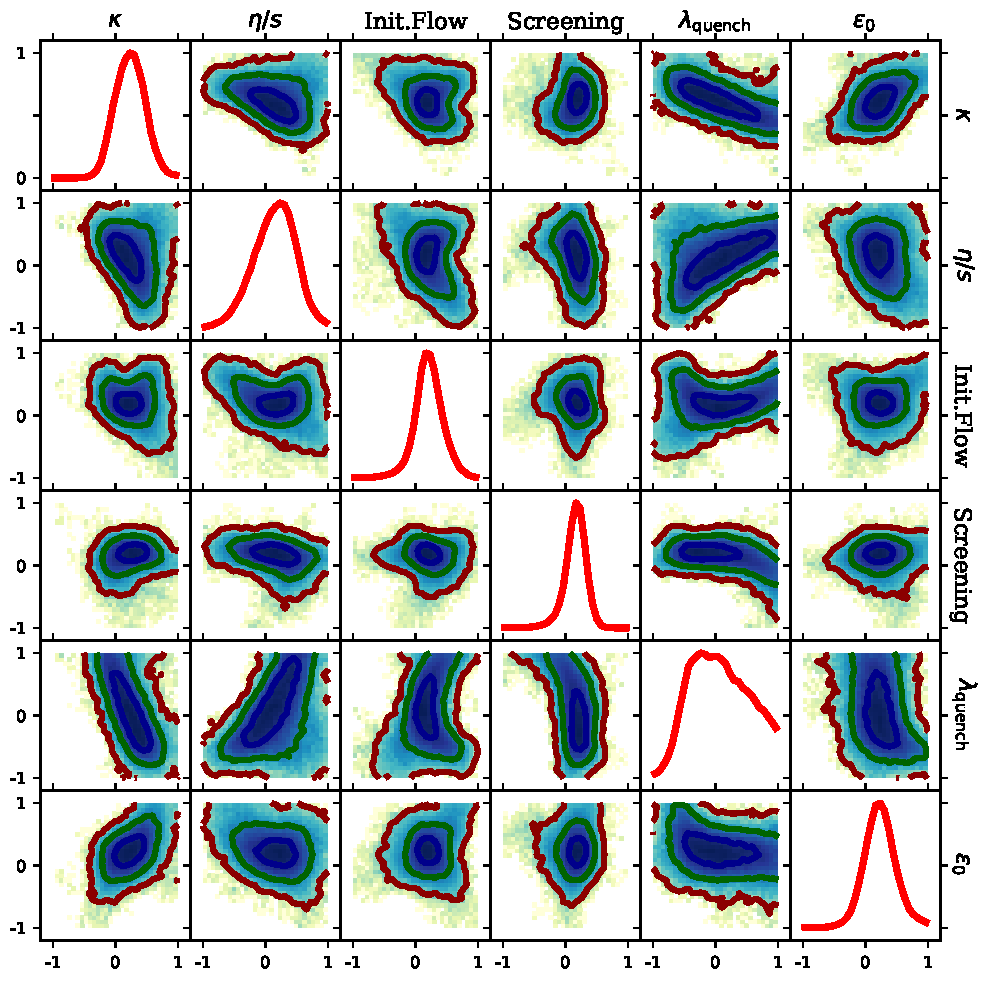
\includegraphics[width=4.5in]{posterior_rhic.pdf}}}
~~\parbox{2.0in}{Projections for the posterior likelihood from the MCMC trace. The contour lines represent $1-\sigma$, $2-\sigma$ and $3-\sigma$ likelihoods.}

The likelihood is projected for individual model parameters, or for pairs. The plot is in terms of the scaled variables, $\theta_i$. To translate to the true model-parameter ranges, one can look at the {\tt smooth\_data/Info/modelpars\_info.txt} file, which gives the prior ranges of the model parameters before they are scaled to the -1 to 1 range. The file {\tt figs/directions.txt} shows how the User can alter plot. For example there is a line in the python script, {\tt ParsToPlot=[1,2,3,4,5,0]}, which the User can edit to change the ordering of the model-parameters, and to choose which model parameters are considered.

Similarly, one can plot the resolving power. The User can visit the directory {\tt figs/resolvingpower/}. The User should copy the files {\tt mcmc\_trace/ResolvingPower.txt} and {\tt smooth\_data/Info/modelpar\_info.txt} to this directory, editing the {\tt smooth\_data/Info/modelpar\_info.txt} as was done for the posterior visualization figures described above. The User must also copy over the {\tt smooth\_data/Info/observable\_info.txt} file and edit it in a similar fashion. In the template file is
{\tt
\begin{verbatim}
meanpt_pion          $\langle p_t\rangle_{\pi}$
meanpt_kaon          $\langle p_t\rangle_{K}$
meanpt_proton        $\langle p_t\rangle_{p}$
Rinv                 $R_{\rm inv}$
v2                   $v_2$
RAA                  $R_{AA}$
\end{verbatim}}
The first column should be exactly the same as the first line in the original file. After running the {\tt mcmc} program, the figure can be produced via the command
{\tt
\begin{verbatim}
${MY_PROJECT}/figs/resolvingpower% ln -s ../../smooth_data/mcmc_trace/ResolvingPower.txt .
${MY_PROJECT}/figs/resolving power% python3 RP.py
\end{verbatim}}
The figure should look like:

\parbox{4.0in}{\centerline{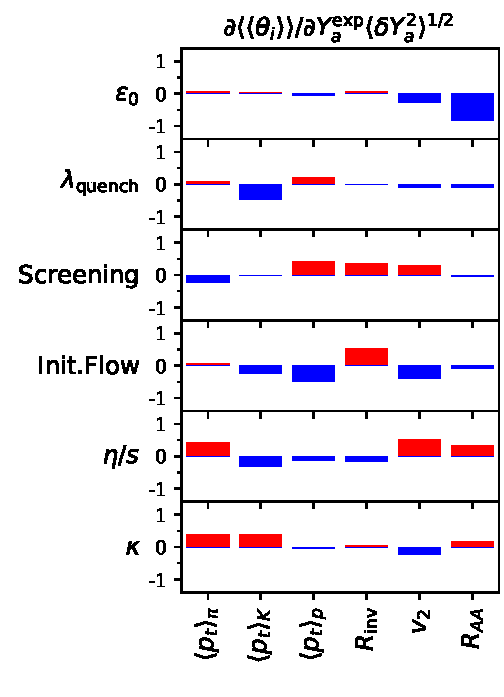
\includegraphics[width=4.0in]{RP_rhic.pdf}}}
\parbox{2.5in}{Resolving Power. Red bars represent positive correlations with $Y^{\rm exp}_a$ and $\theta_i$. Larger bars suggest that the particular observable contributes more to the constraint of the particular model parameter.}

The third provided python script is in {\tt figs/YvY/} and it compares full-model runs (not used for tuning) to the emulator. This is useful for seeing whether the emulator's error estimates are reasonable. First, one must run the program that writes out the emulator predictions for the full-model runs. This is accomplished by the command:
{\tt
\begin{verbatim}
${MY_PROJECT}% smoothy_testvsfullmodelalt
meanpt_pion: 27 out of 50 points within 1 sigma
meanpt_kaon: 41 out of 50 points within 1 sigma
meanpt_proton: 26 out of 50 points within 1 sigma
Rinv: 32 out of 50 points within 1 sigma
v2: 39 out of 50 points within 1 sigma
RAA: 29 out of 50 points within 1 sigma
\end{verbatim}}
If the uncertainty were perfectly stated, 68\% of the points would be within one standard deviation. In this case the fraction was higher, which suggests that the uncertainty was somewhat overstated.

To make the plot, first change into the {\tt figs/YvsY/} directory, and enter
{\tt
\begin{verbatim}
${MY_PROJECT}/figs/YvsY% ln -s ../../fullmodel_testdata .
${MY_PROJECT}/figs/YvsY% python3 YvsY.py
 Observable names:
 ['meanpt_pion', 'meanpt_kaon', 'meanpt_proton', 'Rinv', 'v2', 'RAA']
 Enter iY: 4
 39 of 49  points within 1 sigma
\end{verbatim}}
The script will prompt the User for which observable to consider. In this case, choose 0-5 for the six possible observables. In this case '4' was entered and the chosen observable was the elliptic flow {\tt v2}. 
\parbox{4.5in}{\centerline{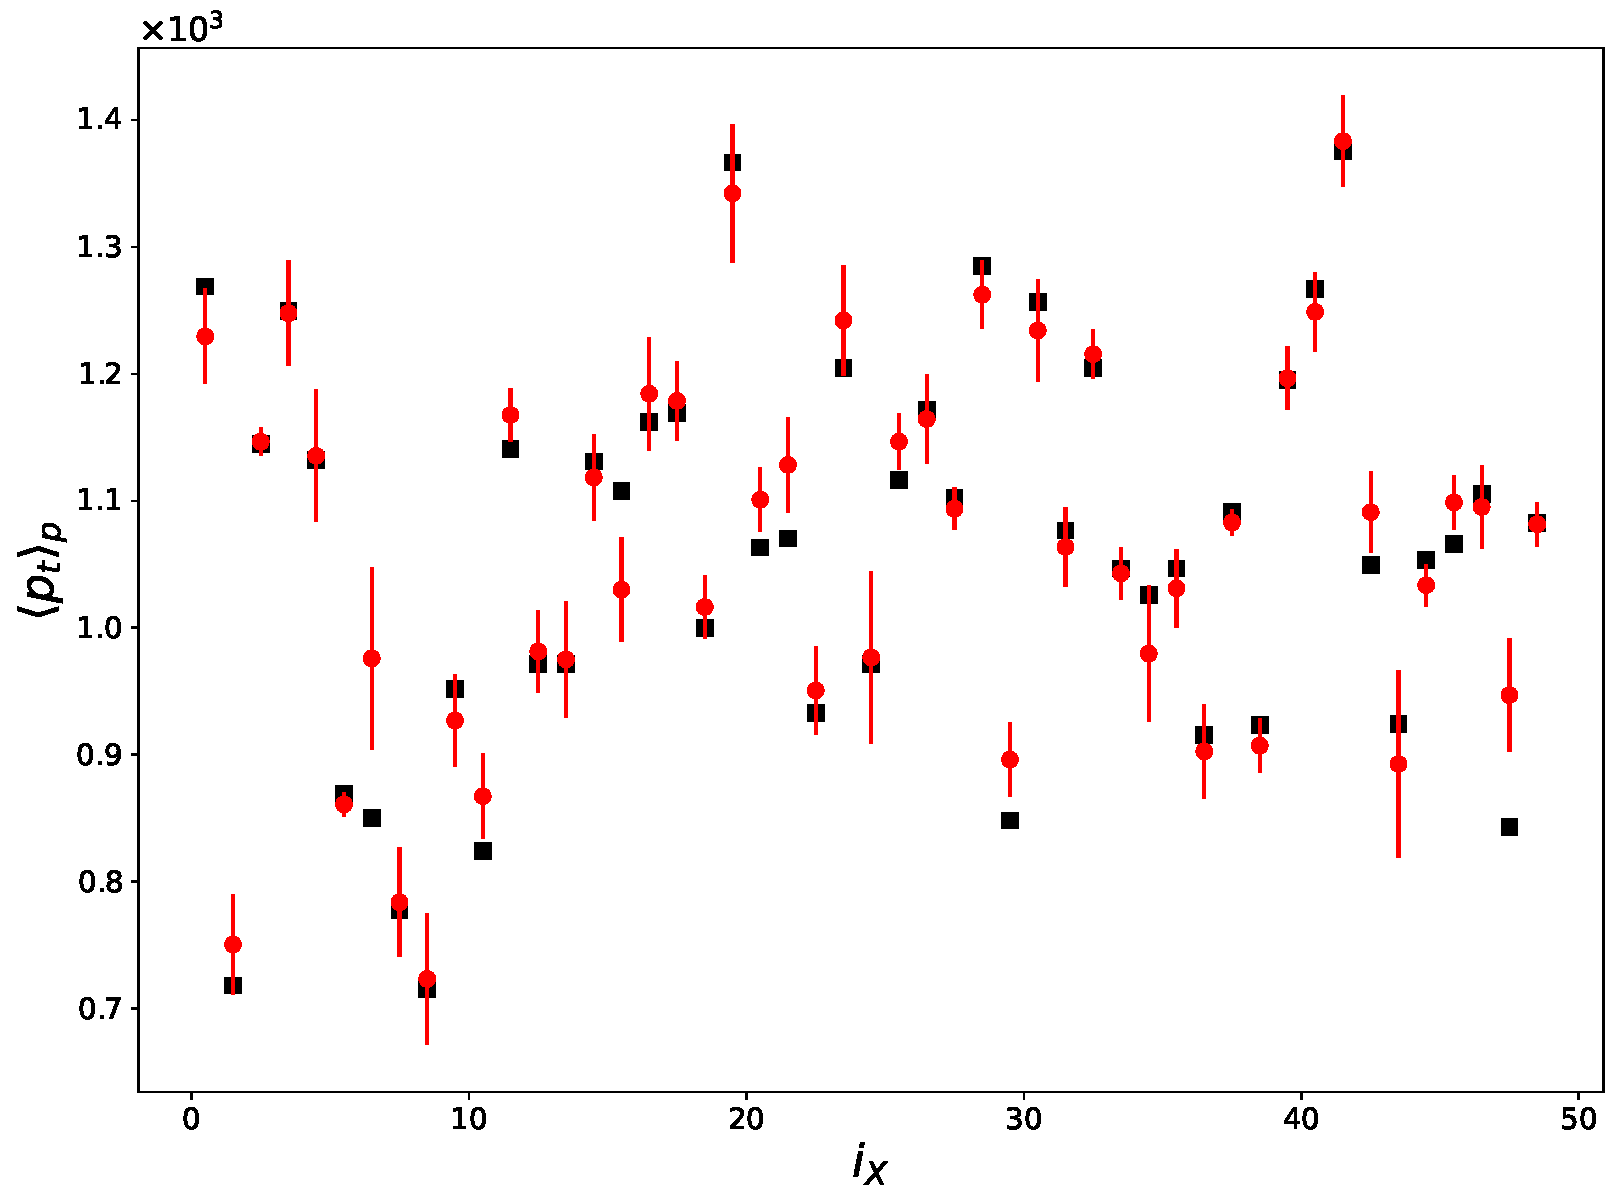
\includegraphics[width=4.0in]{YvsY_rhic.pdf}}}
\parbox{2.25in}{Comparison of full-model values (black squares) for 50 points in parameter space to emulator values (red circles). The uncertainties are solely those associated with the emulation. If the uncertainties were accurately expressed, 68\% of the points would lie within the uncertainty intervals.}

For this example the full-model test data was stored in a few files in the {\tt smooth\_data/fullmodel\_testdata/} directory, consistent with the SURMISE format. Another option would be to use full-model run data stored in the same format and location as the training data. In that case one would invoke the program {\tt smoothy\_testvsfullmodel} (with the {\tt alt}) and the testing runs would be denoted by the {\tt SmoothEmulator\_TestPts} parameter set in the {\tt smooth\_data/smooth\_parameters/emulator\_parameters.txt} file. Those model runs should be chosen separately from those used for training, i.e. those denoted by the {\tt SmoothEmulator\_TrainingPts} parameter.

\subsection{PCA Analysis}
The PCA functionality needs further testing and is not included in the tutorial at this time.

\end{document}
